\documentclass[10pt,oneside,a4paper]{article}
\usepackage[utf8]{inputenc}
\usepackage{amsmath}
\usepackage{indentfirst}
\usepackage{enumitem}
\usepackage[spanish]{babel}
\usepackage[export]{adjustbox}
\usepackage{graphicx}
\graphicspath{ {img/} }
\usepackage{listings}
\usepackage{subfig}
\usepackage{cite}

\addtolength{\oddsidemargin}{-.300in}
\addtolength{\evensidemargin}{-.300in}
\addtolength{\textwidth}{0.600in}
\addtolength{\topmargin}{-.300in}
\addtolength{\textheight}{0.600in} %1.75

\begin{document}
\begin{titlepage}

\title{\Huge Rendering Avanzado  \\[0.7in] \LARGE Iluminación directa\\[3.6in]}
\date{}
\author{Álvaro Muñoz Fernández\\
Iván Velasco González}
\maketitle
\thispagestyle{empty}
\end{titlepage}

\section{Emmiter Sampling}
En esta parte de la practica se debia de implementar en \textit{nori} todo lo necesario para poder realizar un algoritmo de iluminación directa que samplee directamente las fuentes de luz.
\subsection{Mesh Area Light}
\subsubsection{Triangle Sampling}
El primer paso para poder realizar esta tarea consiste en poder samplear de forma correcta una malla de triangulos que modelara nuestra fuente de ilumnación.\\

En primer lugar, se implemento un metodo \textit{sampleTriangle}, el cual obtiene la posición y la normal de un punto interno al triangulo a partir de un sample 2D que se utiliza, por medio de la conversión de distribuciones, como coordenadas baricentricas del triangulo. Sin embargo, esto nos proporciona unicamente dos coordenadas baricentricas, pero a partir de $ u + v + w = 1$, la ultima coordenada se obtiene como $ w = 1 - u - v$. Una vez obtenidas todas las coordenadas baricentricas se interpola la posición del punto a partir de la posición de los vertices que componenen el triangulo, y se realiza un proceso similar para calcular su normal. Es importante destacar que, en caso de que las mallas que conforman las luces no tengan normales asociadas, el algoritmo dara un error al intentar acceder a estas normales.\\

Una vez podemos samplear un triangulo de forma correcta es necesario elegir que triangulo de toda la malla se ha de escoger para ser sampleado, teniendo en cuenta que la probabilidad de que un triangulo sea sampleado debe ser proporcional al area que tenga este respecto a la malla completa. Para conseguir esta PDF se ha utilizado la clase \textit{DiscretePDF} implementada por \textit{nori}, la cual se ha inicializado añadiendole el area de todos los triangulos en su orden de aparición en la malla y despues se ha normalizado. Una vez tenemos construida esta PDF para samplear un triangulo simplemente se le pide un sample a esta distribución a partir de un nuevo valor aleatorio, distinto que los usados para samplear el triangulo en si, para evitar correlar\textit{ samples}.
\subsubsection{Area Emitter}
En esta parte de la practica se debia rellenar todos los metodos necesarios para poder utilizar en un integrador una luz de area, aprovechando los metodos de sampleo implementados en el apartado anterior. Estos metodos son \textit{sample} \textit{eval} y \textit{pdf}.\\

En primer lugar, se debe tener en cuenta que todos los metodos de esta clase reciben como entrada un \textit{EmitterQueryRecord} el cual es el encargado de almacenar toda la información necesaria para que los metodos de la clase funcionen correctamente.\\

Seguidamente se detallara la implemtación del metodo \textit{sample}. Este metodo es el encargado de, a partir del punto a iluminar y un sample, samplear un punto de la fuente de luz y rellenar todo el \textit{EmitterQueryRecord} de forma consecuente teniendo en cuenta el punto a iluminar y el punto de la fuente de luz sampleado. En primer lugar, se rellena el registro con el punto sampleado y su normal los cuales son obtenidos por medio de una llamada al metodo de sampleo de la malla implementado en el apartado anterior, la pdf del punto sampleado, que se obtiene a partir de la malla. Ademas, tambien se rellena la distancia entre el punto a iluminar y el punto sampleado en la fuente de luz , y el vector incidente desde el punto a iluminar a la fuente de luz.\\

Respecto al metodo \textit{eval}, este es el encargado de a partir de un \textit{EmitterQueryRecord} rellenado de forma correcta, por la función de sample o por otro metodo, delvolver la luz que recibe el punto a iluminar desde el punto de la luz elegido. Teniendo en cuenta que no es necesario realizar ningun \textit{test} de oclusión en esta evaluación, ya que de esto se encargará el integrador, se comprueba si el rayo incidente a la luz procede de la cara trasera del triangulo , ya que , en este caso la iluminación devuelta deberia ser 0. Esto se comprueba por medio del producto escalar entre el rayo incidente y la normal, siendo que si este es mayor que 0 el rayo procede de la cara trasera del triangulo. En caso de que esto no sea asi y el rayo proceda de la cara delantera del triangulo, la iluminación que recibe el punto a iluminar del punto sampleado sera la radiancia atenuada por la distancia es decir $Radiance_p = \frac{Radiance}{Distance^2}$\\

Por ultimo, seria necesario implementar el metodo \textit{pdf}, el cual debe devolver la PDF del punto sampleado respecto a ángulo sólido. Sin embargo, en el  \textit{EmitterQueryRecord} la PDF viene expresada respecto del area, ya que es la forma en la que se ha calculado en la malla que representa la fuente de iluminación. Por lo tanto, para obtener la PDF expresada en ángulo sólido a partir de la PDF expresada respecto al área se ha usado la expresión $p_\Omega(x,xl) = p_S(xl)\frac{||x-xl||^2}{nl\cdot\omega_i}$.\\

\subsection{Integrator}
En esta parte de la práctica se debia implementar un metodo de ilumniación directa, es decir un integrador de \textit{nori}, a partir de la siguiente expresión se iluminación:
$$L_o = Le(x,\omega_o) + \int_\Omega Li(x,\omega_i) * brdf(x,\omega_o,\omega_i)  * \cos\theta_i d\omega_i$$
Teniendo en cuenta que, las direcciones de los rayos incidentes ($\omega_i$) van a ser calculadas por medio de un sampleo de las fuentes de luz de la escena.\\

Para realizar esto, en un primer lugar, se trazadara el rayo de camara y se comprobara si colisiona o no con la geometría de la escena. En caso de que colisione, se obtienen el punto de la colisión y su normal asociada, seguidamente comprobamos si el punto a iluminar pertenece a una fuente de luz. Si esto es asi se construye un \textit{EmitterQueryRecord} , donde la dirección de incidencia a la luz es igual a la dirección del rayo de camara y su distancia viene determinada por la distancia de la camara a la fuente de luz. Aunque de esta parte de la implementación no estamos muy seguros, ya que no se tiene en cuenta la distancia a la camara de ningun otro elemento de la escena, pensamos que esto debe ser asi para que las luces pierdan intensidad en función de su distancia a la camara.\\

En el caso de que el rayo de la camara no interseque con una fuente de luz, pero si con algun elemento de la escena, se sampleara un punto de iluminación de la escena. Para ello se ha usado la función \textit{sampleEmitter} implementada por \textit{nori} la cual nos devuelve una fuente de luz de la escena y su pdf asociada. Seguidamente se realiza el sampleo de un punto concreto de esta fuente de luz obteniendo un \textit{EmitterQueryRecord} que encapsula toda la información del sampleo.\\

Seguidamente se rellena un \textit{BSDFQueryRecord} con los datos obtenidos del sampleo de la luz para obtener el valor de la BRDF en ese punto y con el rayo incidente y saliente dados por, el rayo de camara,y el rayo a la fuente de iluminación respectivamente.\\

Despues debido a que el punto de la fuente de luz ha sido sampleado, es neceario comprobar si el punto a iliminar y el punto de la fuente de iluminación tienen visibilidad entre si , para ello se traza un rayo de sombra en la dirección que une los dos puntos, y se comprueba si el rayo interseca con la luz, si esto es asi los puntos son visibles entre ellos y no lo seran en caso contrario.\\

Por ultimo, con toda la informacion necesaria calculada se procede a calcular la iluminación total en el punto a iluminar aplicando la siguiente expresión, la cual es el estimador de Monte Carlo de la función de iluminación vista al principio de esta sección, teniendo en cuenta que luego \textit{nori} sumara y ponderara las muestras:
 $$L_o = L_e  + \frac{ V * L_i * brdf * \cos{\theta}}{P_{light} * P_{point}}$$ 
Donde $Le$ hace referencia a la luz emitida, por lo que solo tendran las fuentes de luz, $V$ hace referencia a la visibilidad entre el punto a iluminar y la fuente de luz, lo cual es necesario tener en cuenta debido a que el punto de la fuente de luz se ha escogido mediante un sampleo , y por tanto, podria estar ocluido. $Li$ representa la cantidad total de luz incidente, la cual sera la luz directa de las fuentes de luz al tratarse de un metodo de iluminación directa y $P_{light}$ y $P_{point}$ hacen referencia a la pdf de la fuente de luz y a la pdf del punto respecto a esa fuente de luz respectivamente. 
\subsection{BRDF Sampling}
En esta parte de la practica se debia implementar un metodo de ilumación directa muy similar al propuesto en el apartado anteior con la salvedad de que la dirección de los rayos incidentes debian calcularse atendiendo a la \textit{BRDF} del material.\\

Por lo tanto, la primera parte del proceso es similar, en primer lugar se obtienen el punto al iluminar y su respectiva normal , se comprueba si el punto pertenece a un emisor. Pero a lo hora de obtener la dirección del rayo incidente se utiliza la función \textit{sample} de la clase \textit{BSDF}, para obtener un \textit{BSDFQueryRecord} que contiene toda la información relativa al sampleo de esa \textit{BSDF} en concreto, como la orientación del rayo de salida, la pdf de la dirección dada y, por supuesto, el valor en si de la brdf asociado a las dos direcciónes.
T
Una vez obtenido el sampleo de la BRDF se traza un rayo en la dirección obtenida y se comprueba si interseca con una fuente de luz, si esto es asi se rellena un \textit{EmitterQueryRecord} con todos los datos necesarios y se evalua la cantidad de iluminación que recibe el punto de esa fuente de luz. En el caso de que el rayo no interseque con una fuente de luz la iluminación recibida por el punto de luz sera 0 si interca con geometria y la luz proveniente del fondo, sino interseca con nada. Esto afectara de forma negativa a la convergencia como se vera en otro apartado.

Seguidamente una vez tenemos todos los valores necesarios se calcula la siguiente expresión, teniendo en cuenta, como en el caso anterior, que \textit{nori} fusionara estas muestras:
$$L_o = L_e + \frac{Li * brdf *\cos\theta}{P_{dir}}$$
Donde $P_{dir}$ hace referencia a la pdf del rayo generado por la función de sampleo de la BRDF en el punto a iluminar. Notese que, al contrario que en el apartado anterior, no tenemos el termino de visivilidad ($V$), esto es debido a que en el caso anterior el punto de la fuente de luz era obtenido mediante sampleo y por lo tanto podria estar ocluido, en este caso el punto de luz se ha obtenido como la intersección de un rayo con la geometria de la escena, y por lo tanto , no puede encontrarse ocluido.\\

Por ultimo, es necesario tener una serie de consideraciones respectivas a la implementación. En \textit{nori} las BRDF discretas devuelven un valor 0 tanto en la brdf como en la pdf, esto provocaba que los brillos especulares de un espejo no se vieran ya que ponian a 0 la función de iluminación. Para solucionar esto se ha comprobado si la pdf es de tipo discreto y se han asginado tanto al color como a la pdf un valor de 1. Por otro lado, nos hemos encontrado el problema que al samplear la BRDF, a veces, el rayo incidente procedia de la parte trasera del triangulo con el que intersecaba, suponemos que debido a problemas de precisión, devolviendo 0 tanto la pdf como la brdf. Por lo tanto, para solucionarlo se tienen en cuenta estas circustancias y si la pdf devuelta por un sampleo de la brdf, que no sea de tipo discreta, se devuelve una $L_o$ de 0 sin pasar por la ecuación para evitar errores. Un ejemplo de estos puntos puede verse en la figura.

\begin{figure}[!htb]
\centering
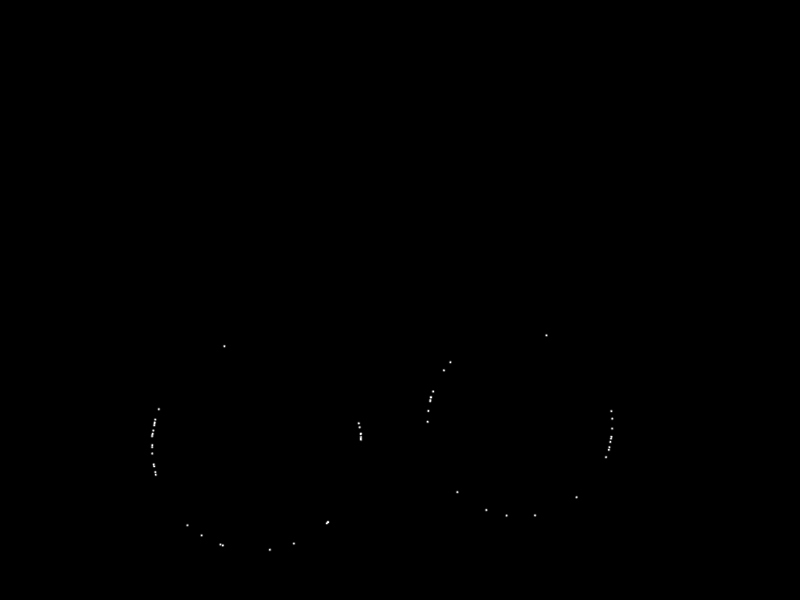
\includegraphics[width=.6\linewidth]{images/pdfs_incorrectas.png}
\caption{Puntos que causan PDFs incorrectas}
\label{fig:disp}
\end{figure}

\subsection{}
  

\end{document}